\section{Modeling of Ablating Thermal Protection Systems}

This section presents the ablation problem for a non-decomposing TPS as a parametrized system of non-linear PDEs. These non-linear PDEs govern the energy of heat conduction and the pseudo-elastic material deformation of the mesh motion. Two different but mathematically-connected numerical solution strategies are provided: (1) a high-fidelity full-order model (FOM) based on a discontinuous Galerkin FEM, and (2) a thermo-elastic RPM based on a one-dimensional approximation to the energy and pseudo-elasticity equations.

\subsection{Governing Equations}

Consider a generic domain $\Omega\subset$, $d=2$ or $3$, illustrated in Fig.~\ref{fig_general_domain}. A heat flux $q_b(x,t)$ is prescribed on the boundary $\Gamma_q$ (i.e., Neumann boundary condition), and the temperature $T_b(x,t)$ is prescribed on boundary $\Gamma_T$ (i.e., Dirichlet boundary condition), where $\Gamma_q\cup\Gamma_T = \partial\Omega$ and $\Gamma_q\cap\Gamma_T = \emptyset$. The ablation occurs only on the heated boundary $\Gamma_q$, and its effects are included into the energy equation using an Arbitrary Lagrangian-Eulerian (ALE) description. The ALE assumes the computational mesh moves with a velocity $\mathbf{v}(x,t)$, which is different to the material velocity, which is set to zero in this work.

\begin{figure}
    \centering
    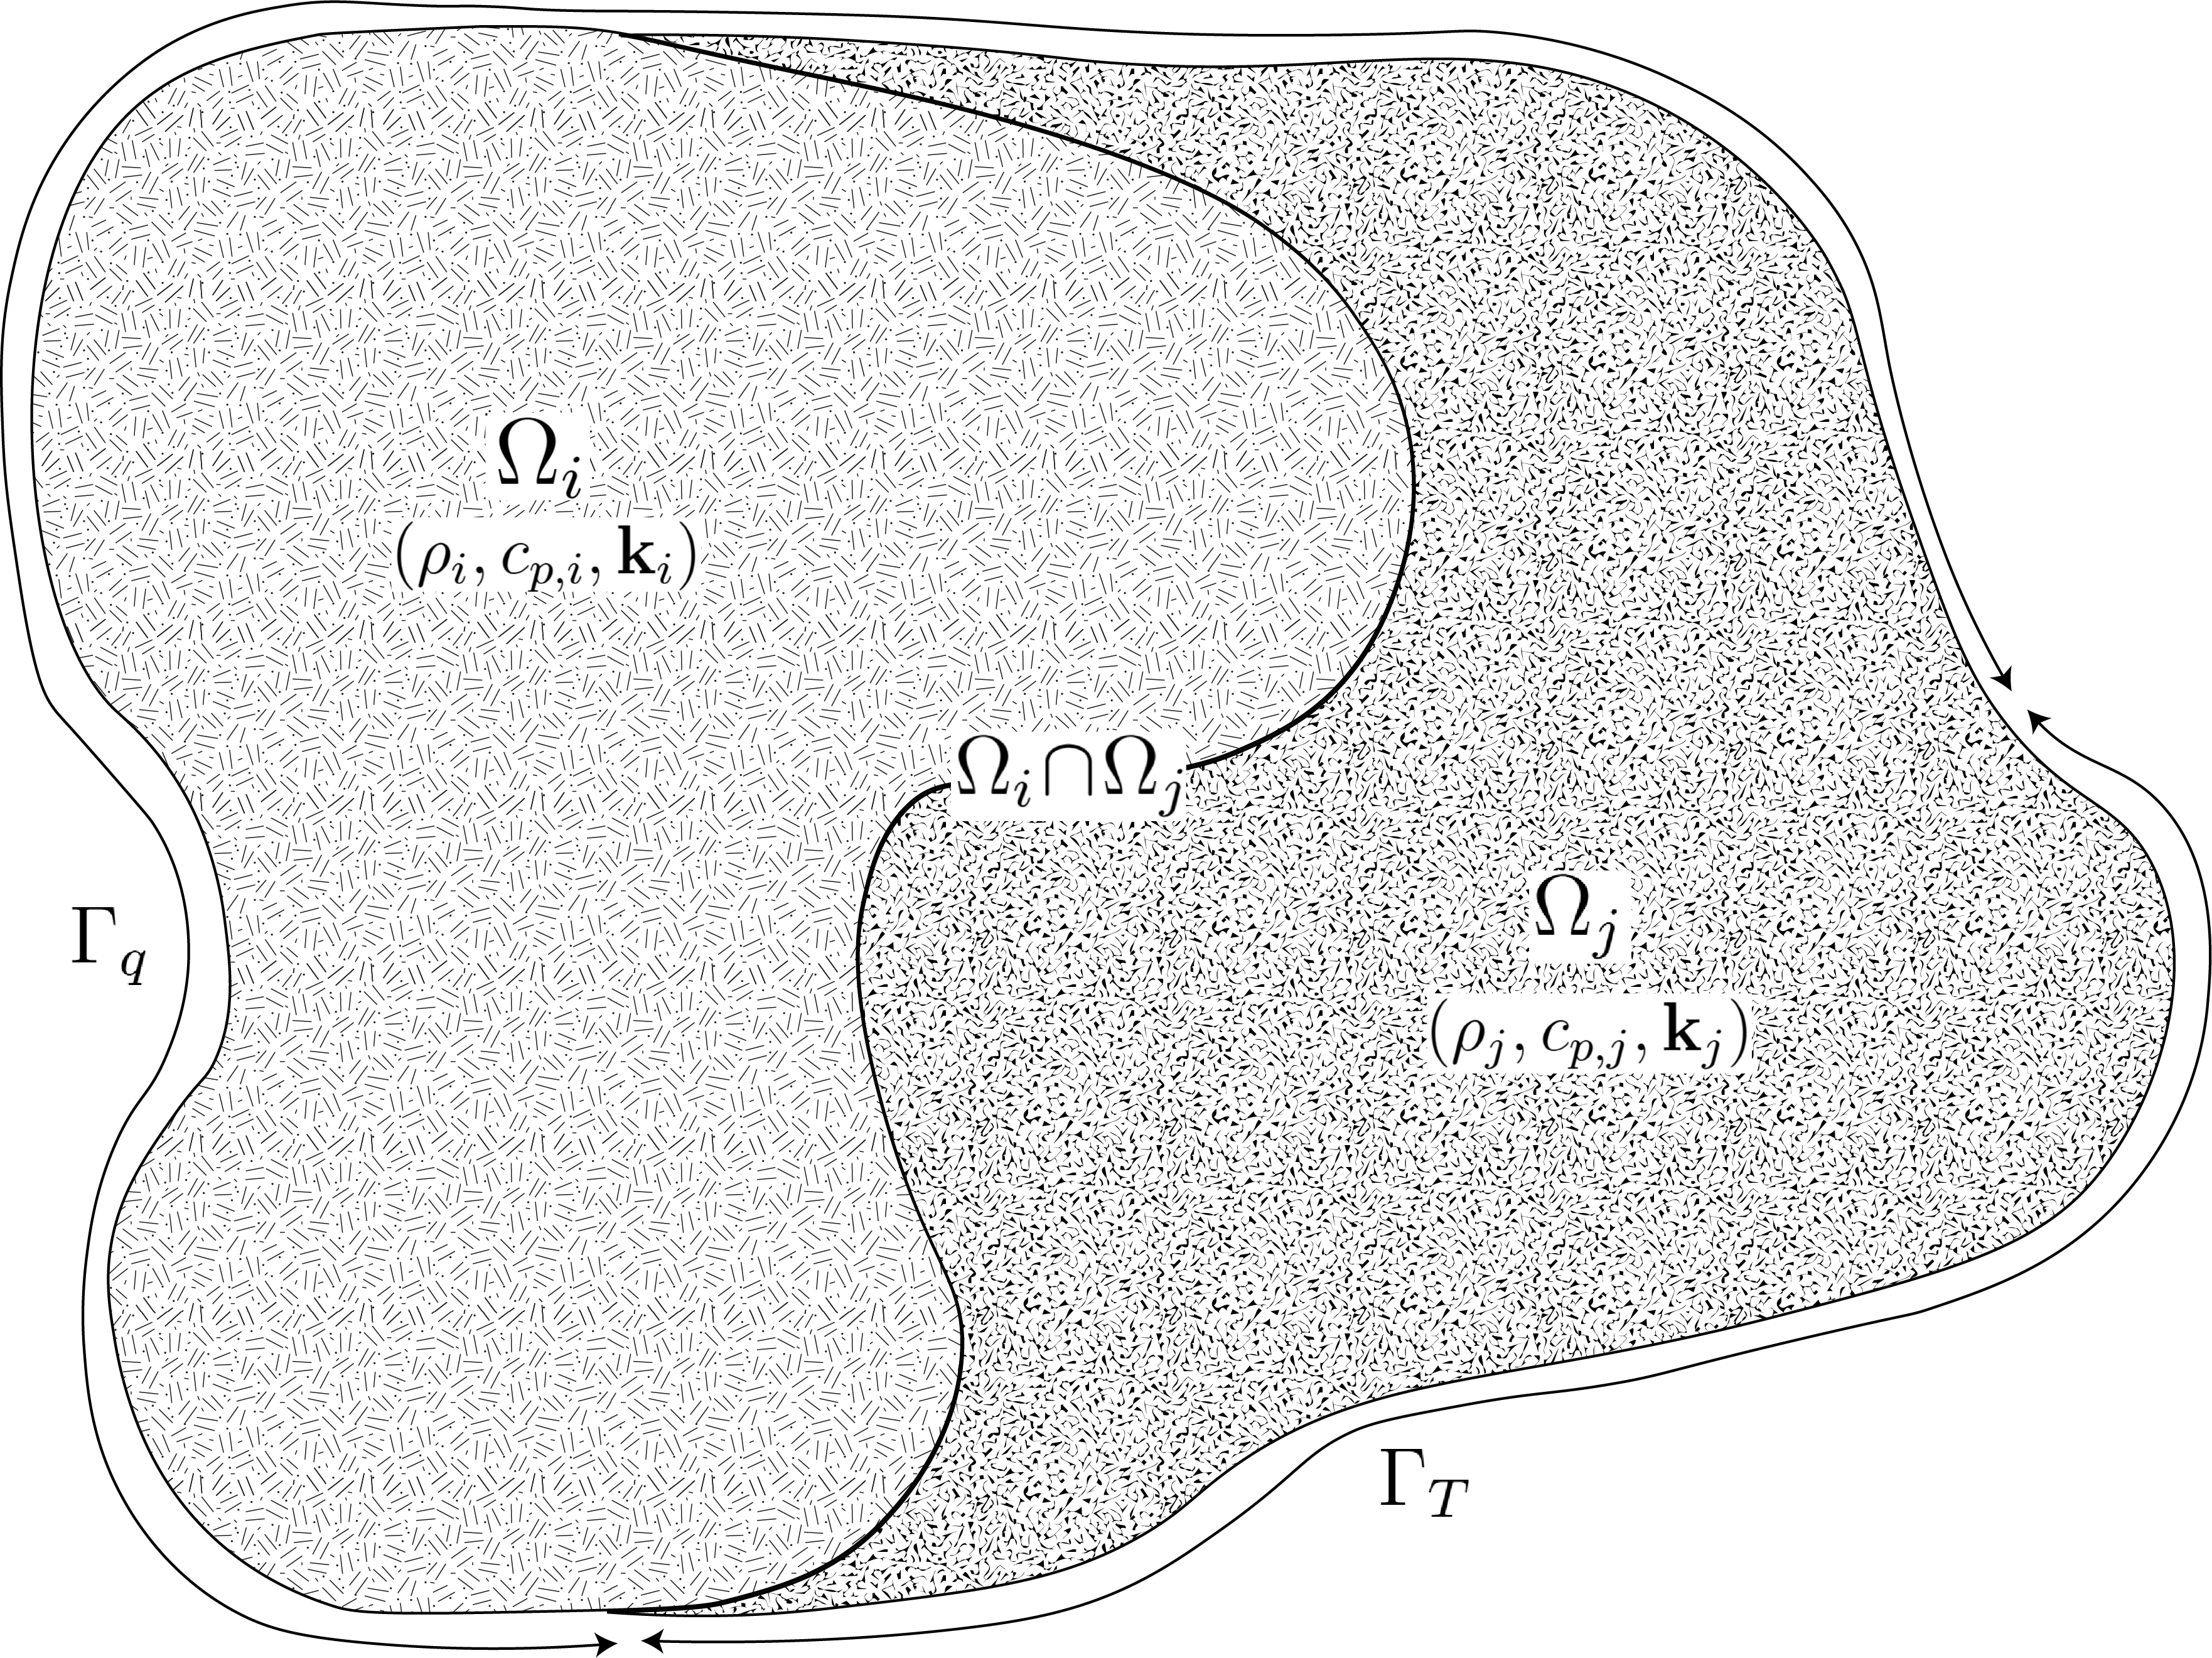
\includegraphics[width=0.6\textwidth]{./figs/general_domain.png}
    \caption{General domain $\Omega$ with prescribed heat flux $q_b(x,t)$ and temperature $T_b(x,t)$ on the boundaries $\Gamma_q$ and $\Gamma_T$, respectively. The mesh moves with a velocity $\mathbf{v}(x,t)$, while the material velocity is $\mathbf{w}(x,t)$.\hl{draw mesh next to arbitrary domain with moving boundaries.}}
    \label{fig_general_domain}
\end{figure}

The transient heat conduction is coupled with the pseudo-elastic mesh motion equation as the following non-linear system of PDEs,
\begin{subequations}
    \begin{align}
        \rho c_p\ppt{T} - \nabla\cdot (\mathbf{k}\nabla T) - \rho c_p\mathbf{v}(x,t)\cdot\nabla T - \cQ(x,t) &= 0,\ x\in\Omega \label{eqn_thermal_pde}\\
        \nabla\cdot\boldsymbol{\sigma}(\mathbf{w}) &= 0\label{eqn_elasticity_pde}
    \end{align}\label{eqn_governing_equations}
\end{subequations}
The density $\rho$ is constant, while the heat capacity $c_p=c_p(T)$ and thermal conductivity $\mathbf{k}=\mathbf{k}(T)\in\mathbb{R}^{d\times d}$ may vary with temperature. The boundary and initial conditions for the heat equation are,
\begin{subequations}
    \begin{align}
        -\mathbf{k}\nabla T\cdot \vn &= q_b(x,t),\ x\in\Gamma_q\label{eqn_thermal_bc_neumann}\\
        T(x,t) &= T_b(x,t),\ x\in\Gamma_T\label{eqn_thermal_bc_dirichlet}\\
        T(x,0) &= T_0(x),\ x\in\Omega\label{eqn_thermal_ic}
    \end{align}\label{eqn_thermal_bc}
\end{subequations}
while for the pseudo-elastic mesh motion, the boundary and initial conditions are,
\begin{subequations}
    \begin{align}
        \bw(x,t) &= \mathbf{w}_q(x,t),\ x\in\Gamma_q\\
        \bw(x,t) &= 0,\ x\notin\Gamma_q\\
        \bw(x,0) &= 0,\ x\in\Omega
    \end{align}\label{eqn_elasticity_bc}
\end{subequations}

The thermo-elastic equations~\cref{eqn_governing_equations}, along with the boundary conditions in \cref{eqn_thermal_bc,eqn_elasticity_bc} are described next. The terms in \cref{eqn_thermal_pde}, in the order they appear, correspond to the unsteady energy storage, heat conduction, temperature advection due to mesh motion, and heat source terms. The \cref{eqn_elasticity_pde} implies that the divergence of the stress tensor $\boldsymbol{\sigma}(\mathbf{w})$ is zero. The stress tensor is related to the strain tensor $\bepsilon(\bw)$ through Hooke's law,
\[
    \boldsymbol{\sigma}(\bw) = \mathbb{D}:\boldsymbol{\epsilon}(\bw)
\]
where $\mathbb{D}$ is the constitutive operator, ``:'' is the double contraction of tensors, and $\bepsilon$ is the symmetric strain tensor given by,
\[
    \bepsilon(\bw) = \frac{1}{2}\left(\nabla\bw + \nabla\bw^T\right)
\]
For instance, an isotropic material assumption results in,
\[
    \bsigma = \lambda\left(\nabla\cdot\bw\right) \mathbf{I} + 2\mu\bepsilon(\bw)
\]
where $\lambda$ and $\mu$ are Lame constants that are arbitrarily selected to model the mesh motion. The ``material'' properties $\lambda$ and $\mu$ can be chosen to tailor the mesh deformation and need not represent the actual material being modeled~\hl{Amar2016}. 

The boundary conditions for the energy equation includes a heated surface (\cref{eqn_thermal_bc_neumann}) and a constant-temperature surface (\cref{eqn_thermal_bc_dirichlet}). The boundary conditions for the pseudo-elasticity equation are a function of the surface temperature $T_q(x,t)$ for $x\in\Gamma_q$ using a B' table. The B' table....
\begin{equation}
    \bw_q(x,t) = \int_{0}^{t} \mathbf{v}(x,\tau)d\tau = \int_{0}^{t}\mathbf{f}\left(T_q(x,\tau)\right)d\tau
\end{equation}


\subsection{Full-Order Model: Discontinuous Galerkin Finite Element Method}

To obtain the full-order numerical solution, the governing equation is spatially discretized using variational principle of Discontinuous Galerkin (DG) to result in a high-dimensional system of ODEs. Note that the choice of DG approach here is mainly for theoretical convenience in the coarse-graining formulation. In Sec.~\hl{x} the full-order TPS ablation simulation is computed using standard FEM instead, and the equivalence between DG and standard FEM is noted upon their convergence.

\subsubsection{Numerical Solution}

\subsubsection{Usage Within an Ablation Simulation}


\subsection{Reduced-Physics Model: One-Dimensional Thermo-Elastic Solver}

In this section,  the thermo-elastic RPM is derived to model the one-dimensional temperature distribution and surface recession for an ablating TPS. The RPM is derived for $N$ non-overlapping inter-connected components $\left\{\Omega_i\right\}_{i=1}^{N}$, as illustrated in Fig.~\hl{x} for $N=2$. The $i$-th component $\Omega_i$ may be associated with a different set of material properties $\left(\rho_i, c_{p,i}, \bk_i\right)$ that are assumed to be continuous within one component, and can be discontinuous across two neighboring components.

The RPM is defined based on two models: (1) a thermal solver based on FEM, and (2) a pseudo-elastic solver for the FEM mesh. The coupling between the thermal and pseudo-elastic solvers is an explicit scheme 


three main components: (1) a thermal solver based on FEM, (2) a pseudo-elastic solver for the FEM mesh, and (3) a lumped capacitance model (LCM) to model the volumetric energy source (i.e., the $\cQ(x,t)$ in \cref{eqn_thermal_pde}) interactions between the inter-connected components.

To start the RPM formulation, consider a partitioning of the general domain in Fig.~\ref{fig_general_domain} into smaller one-dimensional inter-connected material components as illustrated in Fig.~\ref{fig_domain_partition}. Consider the $n$-th component with length $\ell^{(n)}$ illustrated in Fig.~\hl{x}, and for simplicity, assume that the material properties are independent of temperature.

\begin{figure}
    \centering
    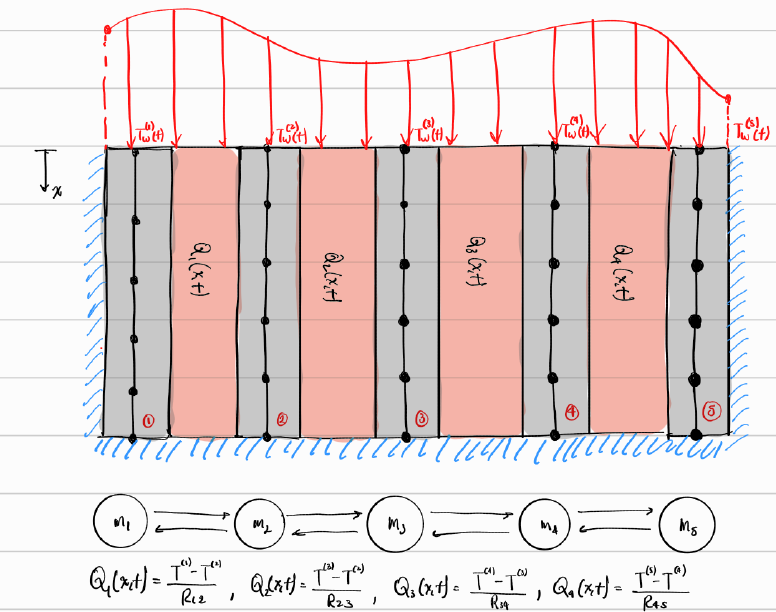
\includegraphics[width=0.5\textwidth]{./figs/domain_partition.png}
    \caption{Partition of the TPS into one-dimensional components.}
    \label{fig_domain_partition}
\end{figure}

For the $n$-th component, the left surface is exposed to the hypersonic flow (Neumann boundary condition), while the right surface is perfectly insulated (adiabatic boundary condition) and no ablation occurs. The left surface is receding with a velocity $v^{(n)}(t)$ that is a function of the surface temperature $T^{(n)}_w(t)=T^{(n)}(0,t)$. This velocity is obtained from a B'-table lookup table,
\[
    v^{(n)}(t) = f(T^{(n)}_w(t))
\]
where $f(\cdot)$ is a cubic spline interpolation of B' and enthalpy tabulated data.

\begin{figure}[h]
    \centering
    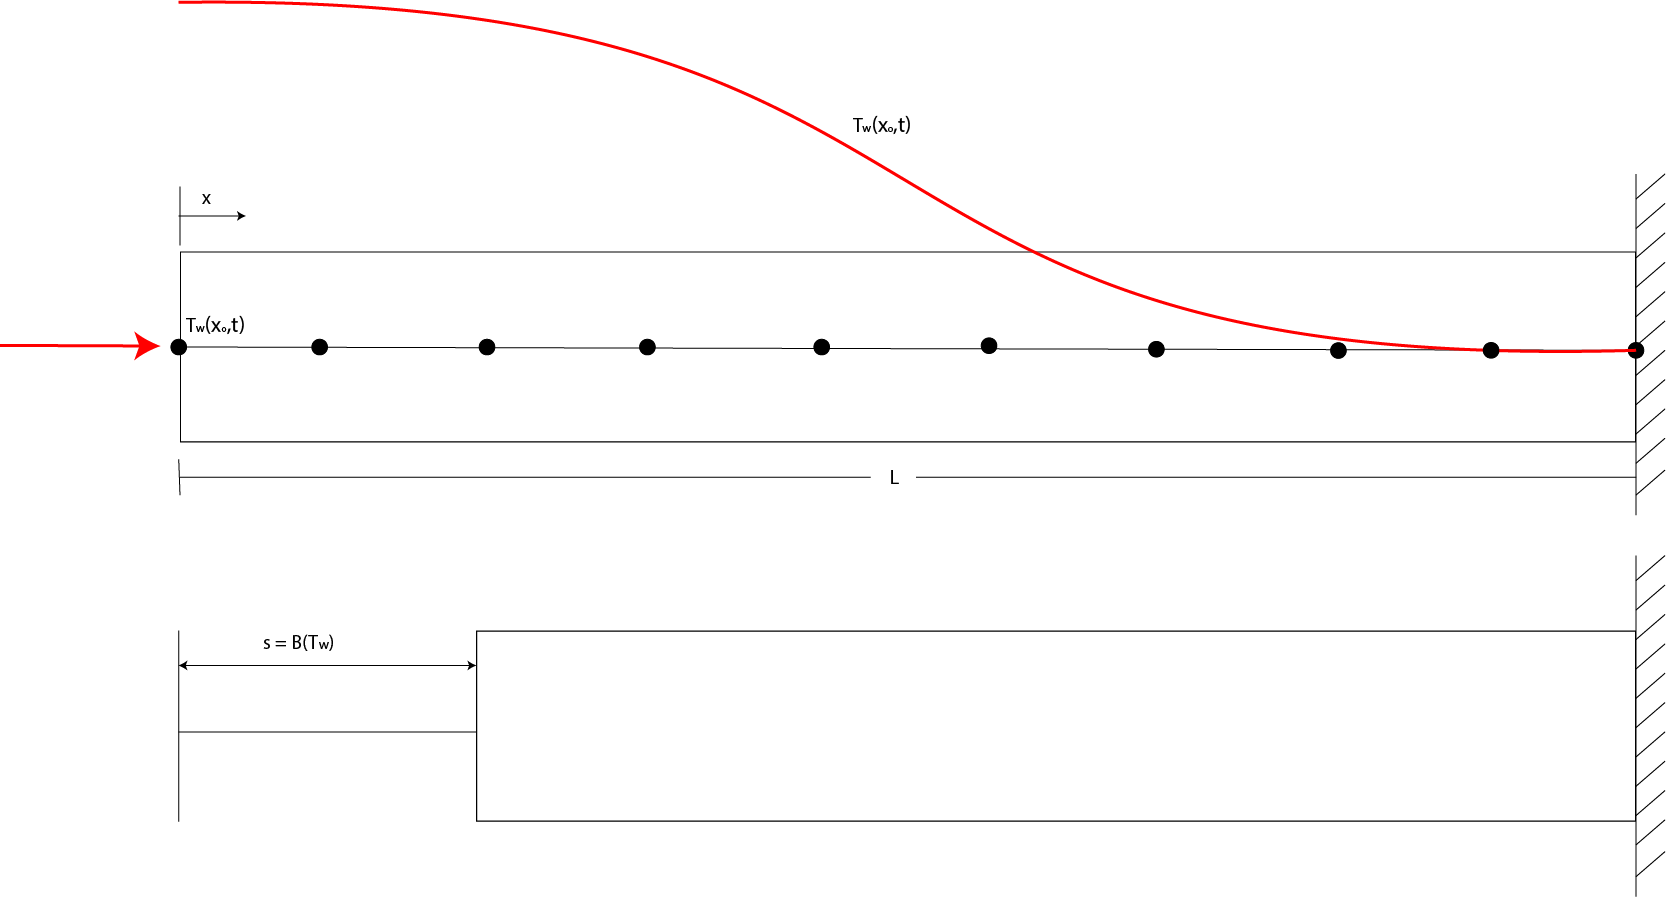
\includegraphics[width=0.9\textwidth]{./figs/ablation.png}
    \label{fig_ablation_domain}
\end{figure}

The governing energy and elasticity equations are defined over the domain $\Omega=[0,\ell]$,
\begin{subequations}
    \begin{align}
        \rho c_p\left(\frac{\partial T^{(n)}}{\partial t} - v^{(n)}(x,t)\frac{\partial T^{(n)}}{\partial x}\right) - \frac{\partial}{\partial x}\left(k\frac{\partial T^{(n)}}{\partial x}\right) - \cQ^{(n,n+1)}(x,t) &= 0\label{eqn_thermal_1d}\\
        \frac{\partial}{\partial x}\left(\frac{\partial u^{(n)}}{\partial x}\right) &= 0\label{eqn_elasticity_1d}
    \end{align}\label{eqn_rpm}
\end{subequations}
with boundary conditions for the energy equation,
\begin{subequations}
    \begin{align}
        -k\frac{\partial T^{(n)}}{\partial x}\Bigg|_{x=0} &= q^{(n)}_b(t)\\
        -k\frac{\partial T^{(n)}}{\partial x}\Bigg|_{x=\ell} &= 0
    \end{align}
\end{subequations}
and for the elasticity equation,
\begin{subequations}
    \begin{align}
        u^{(n)}(0,t) &= \int_{t_0}^{t}v^{(n)}(\tau)d\tau = \int_{0}^{t} f(T^{(n)}_w(\tau))d\tau\\
        u^{(n)}(\ell,t) &= 0
    \end{align}
\end{subequations}

\subsection{Numerical Solution}

Along the one-dimensional domain, a numerical solution based on FEM is adopted for the energy equation, while an analytical solution is adopted for the pseudo-elastic mesh motion. The quasi-steady boundary conditions for the mesh motion are employed via a spline fit to the B' and enthalpy tabulated data as a function of surface temperature. The main results of the numerical approach are presented here and the reader is directed to Sec.~\ref{app_implementation} for details.

\subsubsection{Thermal Solver}

The FEM implementation details are supplied in Appendix~\hl{x}. For the $n$-th component, the result of the FEM discretization is a system of ODEs for the nodal temperatures, coupled to the neighboring component $n+1$ through the energy volumetric source term,
\begin{equation}
    \mathbf{A}^{(n)}\frac{d\mathbf{T}^{(n)}}{dt} + \left(\mathbf{B}^{(n)} - \mathbf{C}^{(n)}(t)\right)\mathbf{T}^{(n)} = \mathbf{f}^{(n,n+1)}(t)
\end{equation}
where,
\begin{itemize}
    \item $\mathbf{A}^{(n)}\in\mathbb{R}^{N\times N}$ is the mass matrix,
    \item $\mathbf{B}^{(n)}\in\mathbb{R}^{N\times N}$ is the stiffness matrix,
    \item $\mathbf{C}^{(n)}(t)\in\mathbb{R}^{N\times N}$ is the advection matrix,,
    \item $\mathbf{T}^{(n)}\in\mathbb{R}^{N}$ is the vector of nodal temperatures, and
    \item $\mathbf{f}^{(n,n+1)}(T)\in\mathbb{R}^{N}$ is the input vector, which incldues the volumetric energy source term $\cQ^{(n,n+1)}(x,t)$.
\end{itemize}
where $N$ is the number of nodes in the one-dimensional mesh for the $n$-th component.

\subsubsection{Pseudo-Elastic Solver}

Note that \cref{eqn_elasticity_1d} is steady. Under the assumption that the mesh deformation is quasi-steady, it can be applied at each time step within an ablation simulation. For instance, a known value of the wall temperature $T_w(t)$ specifies a Dirichlet boundary condition for the displacement, and the resulting nodal displacements within the ablator are determined from \cref{eqn_elasticity_pde}.

Along the one-dimensional domain, the PDE in \cref{eqn_elasticity_pde} simplifies to,
\begin{equation}
    \frac{\partial^2 u}{\partial x^2} = 0
\end{equation}
which has the analytical solution,
\begin{equation}
    u(x,t) = a(t)x + b(t)
\end{equation}
Imposing the boundary conditions leads to,
\begin{equation}
    u(x,t) = u(0,t)\left(1 - \frac{x}{\ell}\right)
\end{equation}
The mesh velocity is the time derivative of the displacement,
\begin{equation}
    v(x,t) = \frac{\partial u(x,t)}{\partial t} = v(t)\left(1 - \frac{x}{\ell}\right)
\end{equation}
which is a function of the wall temperature,
\begin{equation}
    v(x,t) = v(T_w(t)) \left(1 - \frac{x}{\ell}\right)
\end{equation}

\subsubsection{Coupling Scheme}

\subsubsection{Reduced-Physics Ablation Simulation}







